\section{Implementierung SmIdempotencyForwardRecovery}
Die Auswertung der Ergebnisse des SmIdempotencyBackwardRecovery hat gezeigt, dass die Strategie der BackwardRecovery Konsistenz gewährleisten kann. Dabei trat jedoch erneut das Problem des vorzeitigen Abbruchs auf. Das erste Vorkommen eines Netzwerkfehlers innerhalb eines Ts führte zur Kompensierung. Der nächste zu implementierende Zustandsautomat verfolgt zwei Ziele: eine möglichst hohe Erfolgsrate sowie eine möglichst hohe Konsistenz. Mittels ForwardRecovery kann eine Weiterführung der Saga erzwungen werden. Abgebrochen wird lediglich in Zuständen, bei denen ein Ergebnis auftritt, das nicht behebbar ist. 

Für Ts ist lediglich ein Ergebnis wie 409 unbehebbar und es wird zum vorherigen C gewechselt. Für Netzwerkfehler werden Retries eingeführt. Aufgrund der Idempotenz der Teilnehmerservices ist dies problemlos möglich. Nur bei einem eindeutigen Ergebnis wird fortgefahren (200, 208) oder abgebrochen (409). 

Der resultierende Zustandsautomat SmIdempotencyForwardRecovery ist in \cref{fig:SmIdempotencyForwardRecovery} abgebildet.


\begin{figure}[h!]
	\centering
	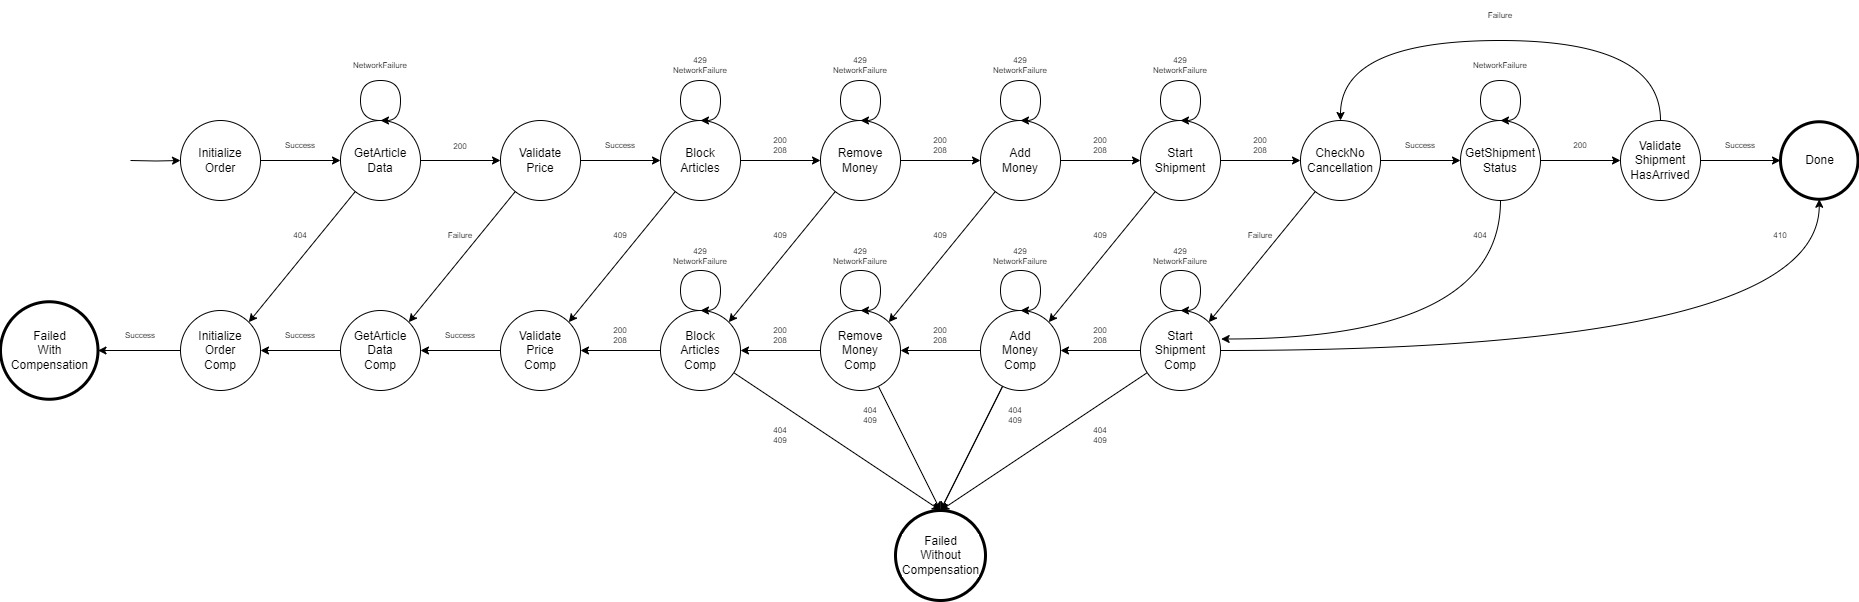
\includegraphics[width=\linewidth]{figures/ChapterVersuchsdurchführung/sm_idempotency_forward_recovery.jpg}
	\caption{DEA für SmIdempotencyForwardRecovery}
	\label{fig:SmIdempotencyForwardRecovery}
\end{figure}
\FloatBarrier

\subsection{StateAnalysisResult}

Das StateAnalysisResult zeigt, dass unabhängig vom Testfall und Testszenario alle Sagas im erwarteten Endzustand münden. 

\paragraph*{Testfall FinishOrders} \mbox{}\\

\begin{center}
	\fontsize{9}{12}\selectfont
	\begin{longtable}[h]{|p{5cm}|p{1cm}|p{1cm}|p{1cm}|}
		\hline
		Messwert & S1 & S2 & S3 \\ \hline
		\endhead
		%\label{tab:smbasic_stateanalysisresult_finishorders}
		\endfoot
		successfull\-Percentage & 1.0 & 1.0 & 0.91 \\ \hline
		finished\-Percentage & 1.0 & 1.0 & 1.0 \\ \hline
		pending\-Percentage & 0.0 & 0.0 & 0.0 \\ \hline
		failedWithCompensation\-Percentage & 0.0 & 0.0 & 0.0 \\ \hline
		failedWithoutCompensation\-Percentage & 0.0 & 0.0 & 0.1 \\ \hline
		hasCorrectEndstate\-Percentage & 1.0 & 1.0 & 1.0 \\ \hline
		containsAllExpectedLogs\-Percentage & 1.0 & 1.0 & 1.0 \\ \hline
		isSuccessfullTestInstance\-Percentage & 1.0 & 1.0 & 1.0 \\ \hline
	\end{longtable}
\end{center}
\FloatBarrier

\paragraph*{Testfall CancelOrders} \mbox{}\\

\begin{center}
	\fontsize{9}{12}\selectfont
	\begin{longtable}[h]{|p{5cm}|p{1cm}|p{1cm}|p{1cm}|}
		\hline
		Messwert & S1 & S2 & S3 \\ \hline
		\endhead
		%\label{tab:smbasic_stateanalysisresult_finishorders}
		\endfoot
		successfull\-Percentage & 0.0 & 0.0 & 0.0 \\ \hline
		finished\-Percentage & 1.0 & 1.0 & 1.0 \\ \hline
		pending\-Percentage & 0.0 & 0.0 & 0.0 \\ \hline
		failedWithCompensation\-Percentage & 1.0 & 1.0 & 1.0 \\ \hline
		failedWithoutCompensation\-Percentage & 0.0 & 0.0 & 0.0 \\ \hline
		hasCorrectEndstate\-Percentage & 1.0 & 1.0 & 1.0 \\ \hline
		containsAllExpectedLogs\-Percentage & 1.0 & 1.0 & 1.0 \\ \hline
		isSuccessfullTestInstance\-Percentage & 1.0 & 1.0 & 1.0 \\ \hline
	\end{longtable}
\end{center}
\FloatBarrier

\subsection{TransactionAnalysisResult}
In \cref{asd} sind die TransactionAnalysisResults für beide Testfälle dargestellt. Es ist erkennbar, dass die Konsistenz in beiden Testfällen für alle Testszenarios eingehalten wird. 

\begin{center}
	\fontsize{9}{12}\selectfont
	\begin{longtable}[h]{|p{2cm}|p{1cm}|p{1cm}|p{1cm}|}
		\hline
		 & S1 & S2 & S3 \\ \hline
		\endhead
		%\label{tab:smbasic_stateanalysisresult}
		\endfoot
		FinishOrders & 1 & 1 & 1 \\ \hline	
		CancelOrders & 1 & 1 & 1 \\ \hline
	\end{longtable}
\end{center}
\FloatBarrier